% ================================================================= CINC 2013 TOÀN BỘ 75 BẢN GHI
\subsubsection{PhysioNet/CinC 2013: 60 bản ghi sạch, không phải 75}
\label{sec:cinc75}

\begin{canhbao}[title={RÚT LẠI (bản 3.5, vòng 7): mọi con số CinC 2013 trên 75 bản ghi trong mục này}]
\textbf{Sự kiện.} Tập set-a của PhysioNet/CinC 2013 \textbf{không độc lập} với ADFECGDB. \textbf{Như ban tổ
chức đã ghi nhận} [Silva và cs., CinC 2013;40:149--152, Bảng 1: ``Abdominal and Direct FECG --- 25'';
Clifford và cs., Physiol Meas 2014;35:1521, Bảng 2], 25 trong 447 bản ghi của Challenge được cắt từ
ADFECGDB, và Clifford và cs.\ (2014) đã cảnh báo rằng một thuật toán dự thi huấn luyện trên ADFECGDB
``may have led to a bias in the results as this database was included in set-a, set-b (and possibly a few
records in set-c)''. Câu đó nằm ngay trong ghi chú đọc bài của nhóm (Bảng bài học, mục p20) và nhóm
\textbf{đã bỏ sót} nó khi viết bản 3.4. Đây \textbf{không} phải phát hiện của nhóm.

\textbf{Phần nhóm đo được} (\texttt{analysis/dulieu\_audit.py}, cài đặt độc lập thứ hai
\texttt{analysis/dulieu\_m4b\_verify.py}): không tài liệu nào cho biết \emph{bản ghi set-a nào} là ADFECGDB;
bằng tương quan chéo chuẩn hoá trên tín hiệu thô, đúng \textbf{15/75 bản} --- a03, a04, a05, a08, a12, a13,
a14, a15, a17, a19, a20, a22, a23, a24, a25 --- là bản sao nguyên văn (NCC $= 1{,}0000$ cả 4 kênh đúng thứ
tự, $|\Delta$RR$| = 0{,}0$\,ms) của các cửa sổ 0--60, 120--180, 240--300\,s của r01, r04, r07, r08, r10; 60
bản còn lại có NCC tối đa 0,62. Vì mọi mô hình của nhóm huấn luyện trên chính 5 sản phụ đó, các con số
75 bản bị thổi phồng \textbf{3,27--7,18 điểm F1}.

\textbf{Số đúng, 60 bản sạch} (\texttt{benchmark\_dpss/eval\_cinc60\_sach.json}, bootstrap 10.000 lần theo
bản ghi, seed 0):
\begin{center}\small
\begin{tabular}{@{}L{4.2cm} C{1.5cm} C{1.5cm} C{1.6cm} C{2.6cm} C{1.5cm}@{}}
\toprule
\textbf{Quy tắc chọn kênh} & \textbf{5 ca} & \textbf{22 ca} & \textbf{Hiệu số} & \textbf{KTC 95\%} & \textbf{T/Th/H} \\
\midrule
\textbf{PSD mù nhãn (khai báo trước)} & 64,04 & \tot{74,28} & $+10{,}24$ & $[+7{,}13;\ +13{,}60]$ & 52/3/5 \\
Trung bình 4 kênh & 56,00 & 67,69 & $+11{,}69$ & $[+9{,}03;\ +14{,}37]$ & 58/2/0 \\
Kênh 0 cố định (hậu kiểm, đã rút) & 48,43 & 61,78 & $+13{,}35$ & $[+9{,}67;\ +17{,}10]$ & 50/--/-- \\
Oracle (dùng nhãn) & 72,76 & 83,60 & $+10{,}84$ & $[+7{,}55;\ +14{,}37]$ & 49/--/-- \\
\texttt{peakprob} (hậu kiểm, giả thuyết) & --- & 82,01 & $+7{,}73$ so PSD & $[+3{,}82;\ +12{,}41]$ & 19/6/35 \\
\midrule
PSD, 53 bản (loại 7 bản nhãn sai) & 64,19 & \tot{75,27} & $+11{,}08$ & $[+7{,}54;\ +14{,}82]$ & 46/2/-- \\
\bottomrule
\end{tabular}
\end{center}
Mô hình 22 ca: 33/60 bản $\geq 90$, 16/60 bản $< 50$, trung vị 95,07; PSD kém oracle \textbf{9,32} điểm
$[+5{,}10;\ +14{,}15]$ và chỉ chọn trúng kênh oracle ở 17/60 bản. Power-MF đơn kênh trên 60 bản sạch: 55,97.
Quy tắc \texttt{peakprob} (+7,73, $p_{\text{Holm}} = 0{,}0039$ trên 7 quy tắc khai báo) được chọn \emph{sau}
khi nhìn kết quả; quy tắc chỉ định trước (\texttt{gate}, +6,44) \textbf{trượt} Holm ($p = 0{,}051$); trên
thang logit quy tắc đứng đầu là \texttt{gate4}; và \textbf{không có bộ dữ liệu công khai thứ ba có nhãn fQRS
thật} để xác nhận (NIFEADB, NInFEA không có nhãn; \texttt{.qrs} của nifecgdb là nhịp mẹ; set-b chưa công bố
nhãn --- \texttt{analysis/XACNHAN.md}). Vì vậy \texttt{peakprob} là \textbf{giả thuyết mạnh, chưa xác nhận}.

\textbf{Các bảng và hình còn lại của mục này giữ nguyên số trên 75 bản ghi để đối chiếu; mọi con số 71,21 /
79,40 / 86,87 / 74,09 / 69,33 / 80,70 / +8,18 / +7,47 / 22/75 trong đó đều ĐÃ RÚT.} Kết luận định tính (thêm
dữ liệu giúp; quy tắc chọn kênh mất giá trị ngoài miền; vẫn còn 16 bản dưới 50) không đổi; các số trong
\S\ref{sec:powermf}, \S\ref{sec:model22} và phần phản biện dùng 75 bản cũng đọc theo hộp này.
\end{canhbao}

\begin{canhbao}[title={(Bản 3.4) Nhóm thay toàn bộ con số CinC 2013 của bản v3.2 --- các số 75 bản dưới đây đã rút ở bản 3.5}]
Mọi con số CinC 2013 trong các bản đề cương trước --- 59,15 / 69,31 / 77,34 / 90,34 --- đều đo trên
\textbf{mẫu 10 bản ghi} (a01--a10) của tập set-a, trong khi set-a có \textbf{75 bản ghi}. Nhóm đã chạy
toàn bộ 75 bản ghi (\texttt{benchmark\_dpss/eval\_cinc75.py} $\to$ \texttt{eval\_cinc75.json}).
\textbf{Mẫu 10 bản ghi bị lệch, và lệch theo hai hướng ngược nhau tuỳ quy tắc chọn kênh.} Con số chính
mới là \textbf{79,40}.
\end{canhbao}

\paragraph{Quy tắc khai báo trước khi chạy.} Hai biến thể được khai báo \textbf{trước} khi chạy:
toàn bộ \textbf{75} bản ghi, và \textbf{68} bản ghi sau khi loại a33, a38, a47, a52, a54, a71, a74 ---
bảy bản ghi mà Behar, Oster và Clifford (CinC 2013;40:297--300) xác định là có chú thích tham chiếu sai.
Nhóm báo cáo cả hai để không ai phải tin vào một lựa chọn loại trừ hậu kiểm.

\begin{table}[H]\centering\small
\caption{PhysioNet/CinC 2013 set-a, zero-shot, toàn bộ 75 bản ghi. Hiệu số là mô hình 22 ca trừ mô hình
5 ca; KTC 95\% bootstrap 10.000 lần, seed 0. Hàng in đậm là \textbf{số chính}: quy tắc chọn kênh mù nhãn
theo mật độ phổ công suất.}
\label{tab:cinc75}
\begin{tabular}{@{}L{3.9cm} C{1.7cm} C{1.7cm} C{1.4cm} C{2.5cm} C{1.5cm} C{1.6cm}@{}}
\toprule
\textbf{Quy tắc chọn kênh} & \textbf{5 ca} & \textbf{22 ca} & \textbf{Hiệu số} &
\textbf{KTC 95\% bootstrap} & \textbf{T/Th/H} & \textbf{Cliff $\delta$} \\
\midrule
\textbf{PSD mù nhãn (chính)} & \textbf{71,21} & \tot{79,40} & $+8{,}18$ & $[+5{,}62;\ +11{,}09]$ &
53/5/17 & 0,232 \\
Kênh 0 cố định (hậu kiểm) & 58,72 & 69,33 & $+10{,}61$ & $[+7{,}46;\ +13{,}98]$ & 52/11/12 & 0,224 \\
Trung bình 4 kênh & 64,78 & 74,09 & $+9{,}31$ & $[+7{,}03;\ +11{,}75]$ & 59/8/8 & 0,176 \\
Oracle (dùng nhãn thật) & 78,21 & 86,87 & $+8{,}66$ & $[+5{,}91;\ +11{,}66]$ & 49/5/21 & 0,222 \\
\midrule
\multicolumn{7}{@{}l}{\textit{68 bản ghi (loại 7 bản chú thích sai), quy tắc PSD:}} \\
\textbf{PSD mù nhãn, $n = 68$} & 72,08 & \tot{80,70} & $+8{,}62$ & $[+5{,}71;\ +11{,}79]$ & 47/4/17 & 0,248 \\
\bottomrule
\end{tabular}
\end{table}

\begin{table}[H]\centering\small
\caption{Hình dạng phân bố trên 75 bản ghi, quy tắc PSD mù nhãn. Đây mới là thông tin lâm sàng, không
phải trung bình.}
\label{tab:cinc75_dist}
\begin{tabular}{@{}L{6.0cm} C{2.6cm} C{2.6cm}@{}}
\toprule
\textbf{Nhóm bản ghi (trên 75)} & \textbf{Mô hình 5 ca} & \textbf{Mô hình 22 ca} \\
\midrule
F1 $= 100$ (hoàn hảo) & 15 & \tot{28} \\
F1 $\geq 90$ & 42 & \tot{48} \\
F1 trong $[50, 90)$ & 11 & 11 \\
F1 $< 50$ (sụp đổ) & \xau{22} & \xau{16} \\
\midrule
Gộp toàn cục (micro F1) & 73,00 & 79,92 \\
\bottomrule
\end{tabular}
\end{table}

\begin{figure}[H]\centering
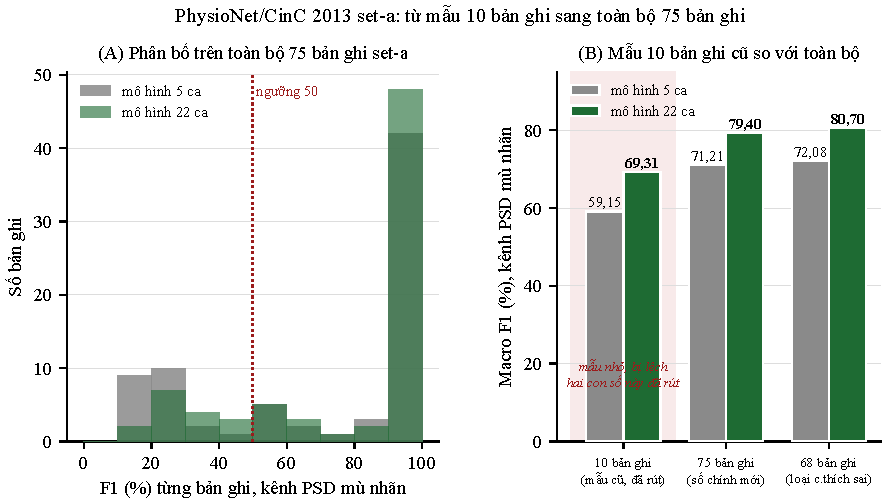
\includegraphics[width=\textwidth]{figs/fig18_cinc75.pdf}
\caption{(A) Phân bố F1 từng bản ghi trên toàn bộ 75 bản ghi set-a --- vẫn \textbf{lưỡng cực}: một đỉnh
ở 90--100 và một đỉnh dưới 30. Mô hình 22 ca đẩy khối lượng sang phải nhưng \textbf{không xoá} đỉnh thấp.
(B) Mẫu 10 bản ghi cũ so với toàn bộ.}
\label{fig:cinc75}
\end{figure}

\subsubsection{Vì sao mẫu 10 bản ghi bị lệch, và lệch theo hai hướng}

Đây là phần nhóm coi là bài học phương pháp quan trọng nhất của đợt này.

\begin{table}[H]\centering\small
\caption{Cùng mô hình 22 ca, cùng checkpoint, cùng bộ chấm --- chỉ đổi \textbf{số bản ghi được
tính}. \xau{Cả hai con số ở cột ``mẫu 10 bản ghi'' (69,31 và 90,34) đều ĐÃ BỊ RÚT} và chỉ giữ lại ở
đây để đối chiếu với con số đúng trên toàn bộ 75 bản ghi.}
\label{tab:cinc_lech}
\begin{tabular}{@{}L{4.6cm} C{3.0cm} C{3.0cm} C{2.6cm}@{}}
\toprule
\textbf{Quy tắc chọn kênh} & \textbf{Mẫu 10 bản ghi \xau{(đã rút)}} & \textbf{Toàn bộ 75 bản ghi} & \textbf{Lệch} \\
\midrule
PSD mù nhãn & \xau{69,31} & \tot{79,40} & \xau{$-10{,}09$} \\
Kênh 0 cố định & \xau{90,34} & 69,33 & \xau{$+21{,}01$} \\
\bottomrule
\end{tabular}
\end{table}

Mười bản ghi a01--a10 \textbf{không} là một mẫu ngẫu nhiên đại diện cho 75 bản ghi:

\begin{enumerate}[leftmargin=1.6em,itemsep=4pt]
\item \textbf{Dưới quy tắc mù nhãn, chúng khó hơn trung bình 10,09 điểm.} Tức bản v3.2 đã
\textbf{báo cáo thấp hơn} năng lực thật của hệ thống. Đây là hướng lệch ít nguy hiểm, nhưng vẫn là lệch.
\item \textbf{Dưới quy tắc kênh 0 cố định, chúng dễ hơn trung bình 21,01 điểm.} Đây mới là chỗ nguy hiểm.
Kênh 0 được chọn \textbf{sau khi} thấy quy tắc PSD thất bại \textbf{trên chính 10 bản ghi đó}. Con số
90,34 vì vậy không chỉ là ``lựa chọn hậu kiểm'' về mặt nguyên tắc --- nó là một siêu tham số đã được
\textbf{khớp vào mẫu đánh giá}, và khi đem ra 65 bản ghi chưa thấy thì nó \textbf{rơi 21 điểm} xuống
69,33, tức \textbf{thấp hơn} cả quy tắc mù nhãn mà nó từng thay thế.
\end{enumerate}

\begin{ghichu}[title={Quy tắc nhóm tự đặt cho mọi kết quả về sau}]
Một quy tắc chọn kênh (hay bất kỳ siêu tham số nào) chỉ được báo cáo nếu nó được \textbf{cố định trước
khi nhìn tập đánh giá}. Con số 90,34 vi phạm điều đó và bị \textbf{rút khỏi mọi bảng chính}; nó chỉ còn
xuất hiện trong \S\ref{sec:cinc75} làm ví dụ về chính lỗi này. Mọi bảng từ đây trở đi dùng
\textbf{79,40 (75 bản ghi, PSD mù nhãn)} làm con số CinC 2013.
\end{ghichu}

\subsubsection{Điều 75 bản ghi nói mà 10 bản ghi không nói được}

\begin{enumerate}[leftmargin=1.6em,itemsep=4pt]
\item \textbf{Sụp đổ xuyên hệ ghi CHƯA được chữa.} Với 75 bản ghi, vẫn còn \textbf{16 bản ghi dưới 50}
(mô hình 22 ca). Kết luận của bản v3.2 --- ``không còn bản ghi nào dưới 50'' --- đúng trên 10 bản ghi và
\textbf{sai} trên 75. Nhóm rút lại kết luận đó. Phân bố vẫn lưỡng cực; đây vẫn là bài toán mở, và vẫn là
lý do đóng góp C3 tồn tại.
\item \textbf{Thêm dữ liệu vẫn giúp, và lần này có đủ mẫu để nói chắc.} $+8{,}18$ điểm với KTC 95\%
$[+5{,}62;\ +11{,}09]$, thắng 53 thua 5 trên 75 bản ghi. Với $n = 75$, đây là kiểm định \textbf{đủ lực},
khác hẳn các so sánh $n = 5$ ở \S\ref{sec:thongke}. Nhưng Cliff $\delta = 0{,}232$ chỉ là hiệu ứng
\textbf{nhỏ}: lợi ích tập trung ở một nhóm bản ghi chứ không nâng đều toàn bộ.
\item \textbf{Quy tắc chọn kênh vẫn là điểm yếu lớn nhất ngoài miền.} Oracle đạt 86,87; quy tắc PSD đạt
79,40. Khoảng cách \textbf{7,47 điểm} chỉ do chọn sai kênh. Trong miền khoảng cách này là 0,02--1,90 điểm.
Quy tắc PSD chọn trúng kênh oracle ở \textbf{22/75} bản ghi (29,3\,\%).
\item \textbf{Loại 7 bản ghi chú thích sai làm mọi con số tốt lên khoảng 1,3 điểm} (79,40 $\to$ 80,70),
không đổi kết luận nào. Nhóm báo cáo 75 bản ghi làm số chính vì quy tắc loại kia dựa trên một nguồn thứ
cấp mà nhóm chưa tự kiểm chứng.
\end{enumerate}
